\documentclass[10pt,a4paper]{article}
\usepackage[margin=2cm]{geometry}
\usepackage{amsmath,amssymb,booktabs,graphicx,caption,xcolor,float,hyperref,tikz}
\usetikzlibrary{arrows.meta,positioning,calc}
\hypersetup{colorlinks=true,linkcolor=blue!50!black,urlcolor=blue!50!black}
\captionsetup{font=small,labelfont=bf}
\title{\vspace{-1.2cm}\textbf{Steering a swarm that owns a proof}\\[2pt]
\large Simulation 2 (asynchronous activation), setup \texttt{task003-symmetric}}
\author{LLM-free simulator; report of 16 October 2026; runs of 15 October 2026\\
\small Mirrors the Simulation 1 report of the same date: same sections, figures and equations. Same data as the 15 October version, reorganised.}
\date{}
\begin{document}
\maketitle
\vspace{-1cm}

\paragraph{How the simulator works.} The world, \texttt{task\_003}, has three candidate allocations; A0 is the
correct one. Each of 24 agents is given one true fact and reasons as an exact Bayesian: its \emph{belief} is the
exact probability of A0, A1 and A2 given the facts it currently remembers. There are no rounds. Each agent acts
at random times, on average once per time unit: it reads $q$ posts drawn at random from the 48 most recent posts
on a shared \emph{board} (never its own), adds their facts to its memory, recomputes its belief, \emph{votes} by
probability matching (a vote drawn from its belief) and posts one remembered fact that supports its vote. Every
remembered fact is forgotten after a random lifetime (on average a fraction $\rho$ survives one time unit; reading
it again renews it). A \emph{controller} with a target, A0 (truth) or A2 (false), acts at random times at rate
$\lambda_c$ until $t = 30$: it reads $q_c$ recent agent posts and, unless the \emph{vote gate} (at least 75\% of
them from agents voting for its target) or the \emph{proof stop} (its target already proved) silences it, posts
the one fact from its pool that best supports its target, at most 30 messages per episode. Agents continue
alone until $t = 40$. Every episode is run three times with the same random draws: without a controller
(\emph{silent}), with the controller targeting A0 and with the one targeting A2.

\paragraph{The facts at the start.} All facts are true. The agents hold, together, a proof of A0; no single
agent does, and neither pool can prove its target (Table~\ref{tab:facts}).

\begin{table}[H]
\centering\small
\caption{Facts available at $t = 0$ and what each set implies, $P(\text{A0}, \text{A1}, \text{A2} \mid \text{facts})$.}
\label{tab:facts}
\begin{tabular}{lcc}
\toprule
set of facts & facts & $P(\text{A0}, \text{A1}, \text{A2})$ \\
\midrule
agents' facts, all together (24 agents, one fact each) & 18 distinct & (1, 0, 0): proves A0 \\
A0 pool (controller with target A0) & 12, of which 10 new to the agents & (0.963, 0.037, 0) \\
A2 pool (controller with target A2) & 12, of which 10 new to the agents & (0.114, 0, 0.886) \\
agents' facts + either pool & 28 distinct & (1, 0, 0) \\
\bottomrule
\end{tabular}
\end{table}

\paragraph{The runs.} Posts read by an agent $q \in \{3, 6, 12\}$; posts read by the controller
$q_c \in \{3, 6, 12, 24\}$; controller rate $\lambda_c \in \{0.5, 1, 2, 3, 4, 5, 6, 7, 8\}$ (one fact per
message); memory $\rho \in \{1, 0.75, 0.5, 0.25\}$; vote gate on and off; proof stop on; 1{,}000 episodes per
setting (1{,}740 settings). Unless stated otherwise: $q = 6$, $q_c = 12$, $\lambda_c = 1$ (the main setting,
which posts about as many facts as Simulation 1 with one fact per night), gate on. The vote gate is on throughout.

\paragraph{Summary.} The 24 agents together own a proof of A0, and with full memory they keep it: no controller
changes the swarm for more than a few time units. \textbf{Forgetting is what makes the swarm steerable}: the
shorter the memory, the larger the effect, and the false controller wins the majority when $\rho \le 0.5$
(Figure~\ref{fig:votes}). Seen side by side (Figures~\ref{fig:timeseries}, \ref{fig:phaserq}--\ref{fig:phaseqx}),
\textbf{susceptibility and readability move together} (they rise, overshoot, persist and reverse together), while
\textbf{the efficiency $\eta$ hardly moves} (0.76--0.94): it measures how symmetric the two controllers' effects are,
not how large. \textbf{The 30-message budget sets the end point and the rate sets the speed}: the slope of the
susceptibility against the rate is large early and for the first unit of rate, and close to zero by $t = 30$
(Figures~\ref{fig:strength}, \ref{fig:strengthtime}); per fact, slow control is the most effective
(Figure~\ref{fig:perfact}). \textbf{Reading more posts protects the proof when agents remember and helps the
controller when they forget} (Figure~\ref{fig:phaserq}). Every controller replaces part of the agents' own proofs
(Figure~\ref{fig:proofs}).

\section{Quantities}\label{sec:quantities}

\paragraph{Votes.} With $n_{a,t}$ the number of agents whose last vote is answer $a$ at time $t$ and $N_t$ the
number of agents who have voted,
\begin{equation}\label{eq:share}
x_{a,t} = n_{a,t}/N_t .
\end{equation}
At $t = 0$ nobody has voted and we set $x_{a,0} = 0$; all agents have voted by $t \approx 5$. (The 9--14 October reports divided by 24, which counted agents who had
not yet acted as voting against the target; this inflated the apparent rise of the shares and the apparent bias of
the controller's sensing at early times.)

\paragraph{Paired susceptibility.} Following \texttt{BLACKBOARD\_OBSERVABLES\_AND\_EFFICIENCIES} (\S3), for a
controller policy $\pi$ and an answer $a$,
\begin{equation}\label{eq:chi}
\chi^{(a)}_{\pi,t} \equiv G^{(a)}_t(\pi) = \mathbb E\bigl[x^{\pi}_{a,t} - x^{\rm base}_{a,t}\bigr],
\end{equation}
the mean over episodes of the difference between the controlled run and the silent run of the same episode. We
report it on the controller's own target: $G_t \equiv G^{(0)}_t(\pi^{+})$ for the controller targeting A0 and
$G_t \equiv G^{(2)}_t(\pi^{-})$ for the one targeting A2.

\paragraph{Target and state.} The target $Z \in \{\text{A0}, \text{A2}\}$ is drawn by a fair coin. The state $X$
at time $t$ is the vote of a randomly chosen agent, $X \in \{\text{A0},\text{A1},\text{A2}\}$. Each episode $e$ of arm $s$
(silent 0, target A0 $+$, target A2 $-$) contributes its vote shares $y^{(e)}_s(x) = x_{x,t}$, and
\begin{equation}\label{eq:P}
P_s(x) = \frac1E\sum_{e=1}^{E} y^{(e)}_s(x), \qquad E = 1000 .
\end{equation}

\paragraph{Readability and efficiency.} With $Q = \frac12(P_+ + P_-)$ and $\mathrm{KL}(p\Vert q) = \sum_x p(x)\log_2[p(x)/q(x)]$,
\begin{equation}\label{eq:I}
I(Z;X) = \tfrac12\,\mathrm{KL}(P_+\Vert Q) + \tfrac12\,\mathrm{KL}(P_-\Vert Q),
\end{equation}
the information the state carries about the target (at most 1 bit). The controllers' total change from silence
splits exactly into a directed and an undirected part,
\begin{equation}\label{eq:C}
C = \tfrac12\,\mathrm{KL}(P_+\Vert P_0) + \tfrac12\,\mathrm{KL}(P_-\Vert P_0) = I(Z;X) + \mathrm{KL}(Q\Vert P_0),
\end{equation}
and the efficiency is the directed share,
\begin{equation}\label{eq:eta}
\eta = I(Z;X)/C .
\end{equation}
Silence sometimes never shows a value of $X$ that a controller reaches, which would make $C$ infinite. Before
computing any KL, every arm's distribution therefore receives the same pseudo-count of $\alpha = 0.5$ episodes per
value of $X$ ($K$ values),
\begin{equation}\label{eq:smooth}
\tilde P_s(x) = \frac{E\,P_s(x) + \alpha}{E + \alpha K}.
\end{equation}
With $\alpha = 1$ instead, $\eta$ changes by at most 0.004; without it, by at most 0.005 where $C$ is finite. $\eta$ is not defined when $C < 0.01$ bits (no measurable change);
such values are left blank. Equation~(\ref{eq:C}) holds in the data to $4\times10^{-15}$ bits.

\paragraph{Cost.} $F_t$ is the number of facts the controller has posted up to $t$ (mean per episode); the gain
per fact is $G_t/F_t$, and the marginal susceptibility is the slope between neighbouring rates,
\begin{equation}\label{eq:slope}
\frac{\Delta G}{\Delta\lambda_c} = \frac{G(\lambda_c^{(k+1)}) - G(\lambda_c^{(k)})}{\lambda_c^{(k+1)} - \lambda_c^{(k)}} .
\end{equation}

\section{Votes over time}

\begin{figure}[H]
\centering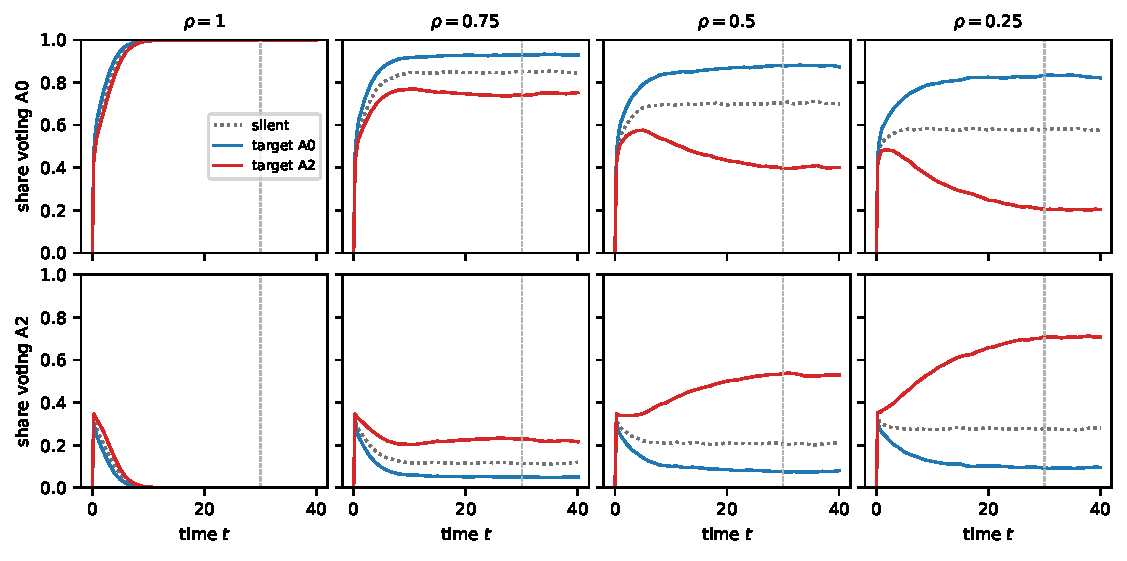
\includegraphics[width=0.95\linewidth]{figures/fig_votes.pdf}
\caption{Share of agents voting A0 (top) and A2 (bottom), Eq.~(\ref{eq:share}), without a controller (dotted),
with the controller targeting A0 (blue) and A2 (red); one column per memory $\rho$. $q = 6$, $q_c = 12$,
$\lambda_c = 1$, gate on. At $t = 0$ nobody has voted and every share is 0; after that the shares count only agents
who have voted (all have by $t \approx 5$). The controller stops at $t = 30$ (dashed). 95\% intervals are narrower
than the lines ($\pm 0.01$).}
\label{fig:votes}
\end{figure}

\begin{itemize}\itemsep1pt
\item \textbf{The shorter the memory, the less firmly the silent swarm holds the truth}: 100\%, 85\%, 71\% and
  58\% vote A0 at $t = 30$ for $\rho = 1, 0.75, 0.5, 0.25$.
\item \textbf{With full memory no controller matters}: every agent votes A0 by $t \approx 10$ in all three arms.
\item \textbf{The false controller wins the majority when $\rho \le 0.5$}: A2 gets 54\% ($\rho = 0.5$) and 71\%
  ($\rho = 0.25$) of the votes, against 21\% and 28\% in silence; at $\rho = 0.75$ only 23\%.
\item \textbf{The truth controller restores the truth} to 84--93\% at every $\rho < 1$.
\end{itemize}

\section{Observables as time series}\label{sec:time}

\begin{figure}[H]
\centering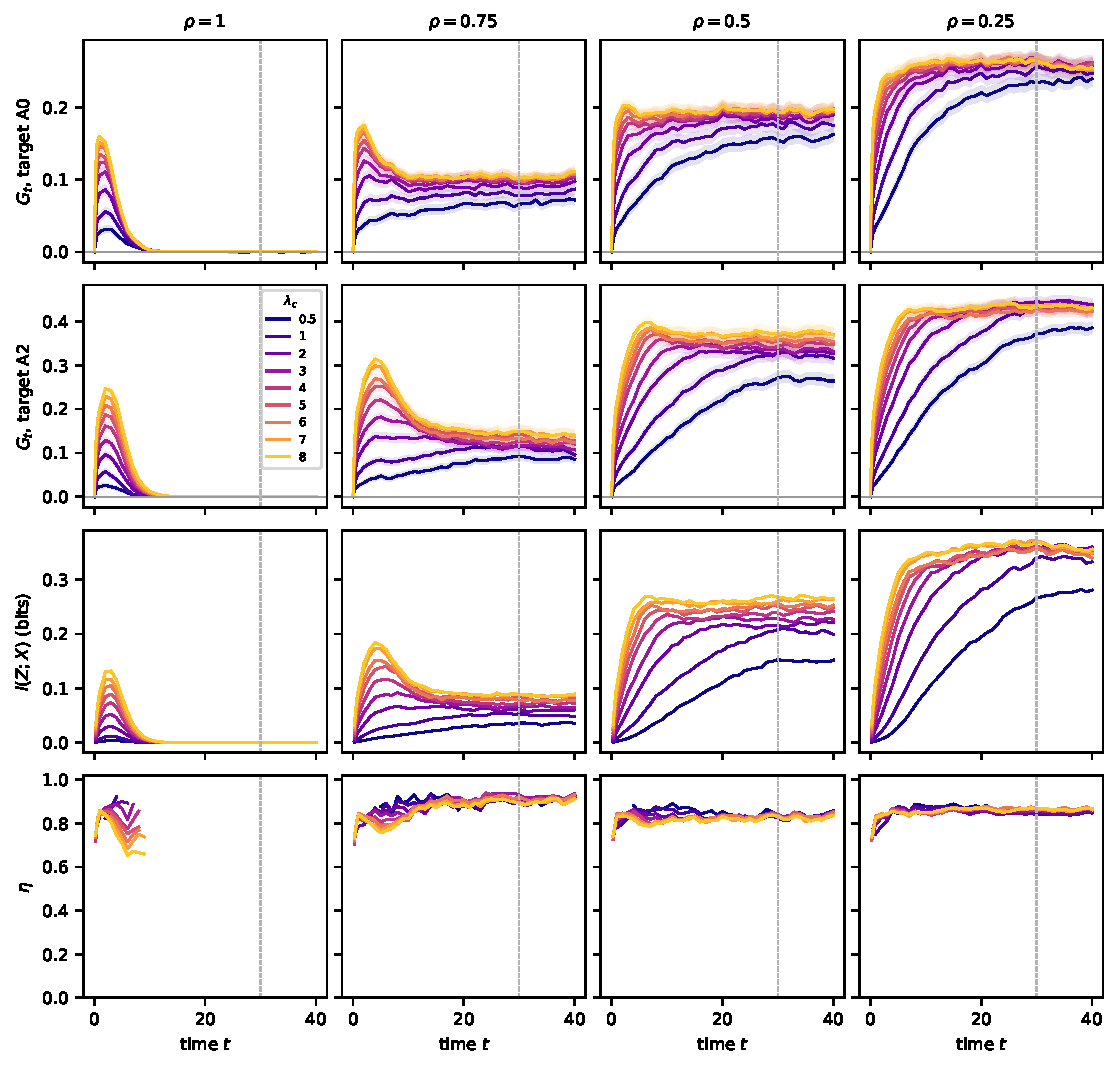
\includegraphics[width=0.95\linewidth]{figures/fig_timeseries.pdf}
\caption{All observables over time, one column per memory $\rho$, one curve per controller rate $\lambda_c$;
$q = 6$, $q_c = 12$, gate on. Rows: paired susceptibility $G_t$, Eq.~(\ref{eq:chi}), for target A0 and target A2
(bands: 95\% intervals; $G_0 = 0$); readability $I(Z;X)$, Eq.~(\ref{eq:I}); efficiency $\eta$, Eq.~(\ref{eq:eta})
(blank: undefined). The controller stops at $t = 30$ (dashed).}
\label{fig:timeseries}
\end{figure}

\begin{figure}[H]
\centering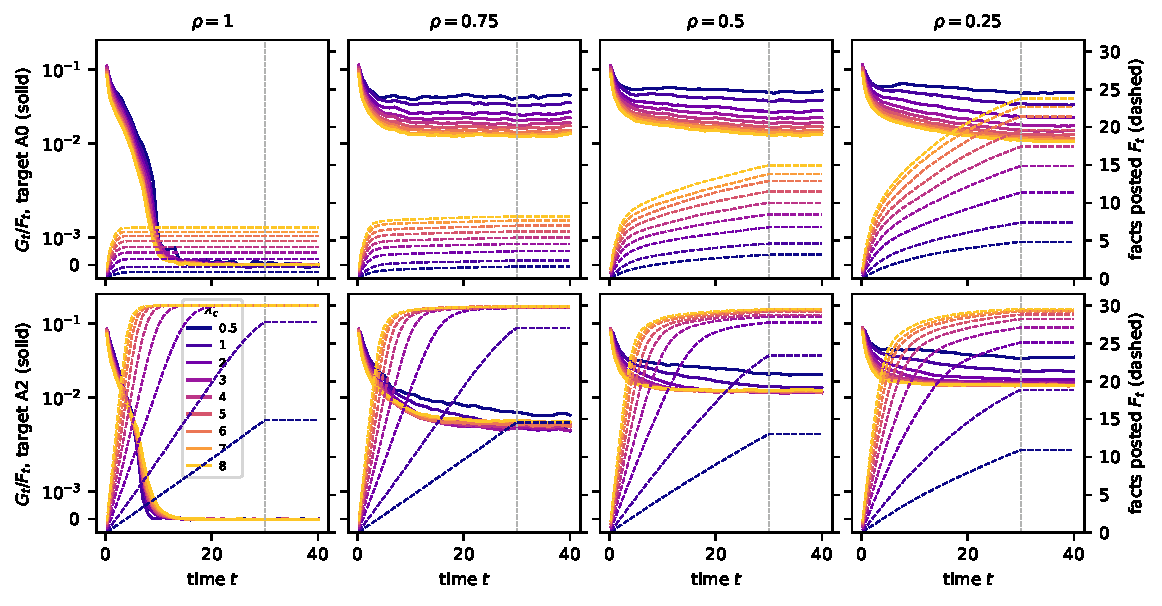
\includegraphics[width=0.95\linewidth]{figures/fig_per_fact.pdf}
\caption{Gain per fact $G_t/F_t$ (solid, left axis, log scale; shown once at least half a fact has been posted)
and facts posted $F_t$ (dashed, right axis), target A0 (top) and A2 (bottom), one colour per rate; $q = 6$,
$q_c = 12$, gate on.}
\label{fig:perfact}
\end{figure}

\paragraph{Susceptibility (Figure~\ref{fig:timeseries}, rows 1--2).}
\begin{itemize}\itemsep1pt
\item \textbf{It grows as memory shortens}: at $t = 30$, target A2, $G = 0.09$--$0.15$ ($\rho = 0.75$),
  $0.27$--$0.37$ ($\rho = 0.5$), $0.37$--$0.44$ ($\rho = 0.25$); target A0, $0.07$--$0.10$, $0.16$--$0.19$,
  $0.23$--$0.26$.
\item \textbf{With full memory it is only transient}: target A2 reaches $0.25$ at $t \approx 2$ ($\lambda_c = 8$)
  and is gone by $t \approx 10$.
\item \textbf{Fast controllers overshoot when agents remember well}: at $\rho = 0.75$, $\lambda_c = 8$, target A2
  peaks at $0.32$ ($t \approx 4$) and relaxes to $0.15$; at $\rho \le 0.5$ the peak is kept.
\item \textbf{It persists after the controller stops}: from $t = 30$ to 40 it changes by at most $0.02$.
\end{itemize}

\paragraph{Readability and efficiency (rows 3--4).}
\begin{itemize}\itemsep1pt
\item \textbf{Readability has the shape of the susceptibility}: it rises, overshoots and persists where $G$ does,
  and is largest at $\rho = 0.25$ ($I = 0.27$--$0.37$ bits at $t = 30$, against $0.04$--$0.09$ at $\rho = 0.75$).
\item \textbf{Efficiency does not}: after $t \approx 3$, $\eta$ stays between $0.76$ and $0.94$ for every rate at
  $\rho < 1$, while $G$ and $I$ vary several-fold. Faster control raises the directed change and the total change together, so their
  ratio does not move; $\eta$ reports the symmetry of the two controllers' effects, not their size.
\end{itemize}

\paragraph{Gain per fact and facts posted (Figure~\ref{fig:perfact}).}
\begin{itemize}\itemsep1pt
\item \textbf{Each fact buys most at the start}: $G_t/F_t$ is largest in the first time units and falls as facts
  accumulate.
\item \textbf{The slowest controller is the most effective per fact}: at $t = 30$, target A2, $\rho = 0.5$:
  $0.021$ per fact at $\lambda_c = 0.5$ (13 facts) against $0.013$ at $\lambda_c = 8$ (30 facts); at $\rho = 0.25$:
  $0.034$ against $0.015$.
\item \textbf{The false controller spends its budget, the truth controller does not}: target A2 reaches the 30-message
  budget by $t \approx 5$ at $\lambda_c = 8$; target A0 posts only 2--24 facts by $t = 30$ because the gate keeps it
  silent once the swarm agrees, which is why it gets more per fact ($0.049$ at $\rho = 0.5$, $\lambda_c = 0.5$).
\end{itemize}

\section{Phase diagrams}\label{sec:phase}

All panels at $t = 30$, gate on; the susceptibility is for target A2 (grey number: its 95\% interval includes 0);
readability and efficiency are for the pair of targets. Colour scales are shared with the Simulation 1 report.

\begin{figure}[H]
\centering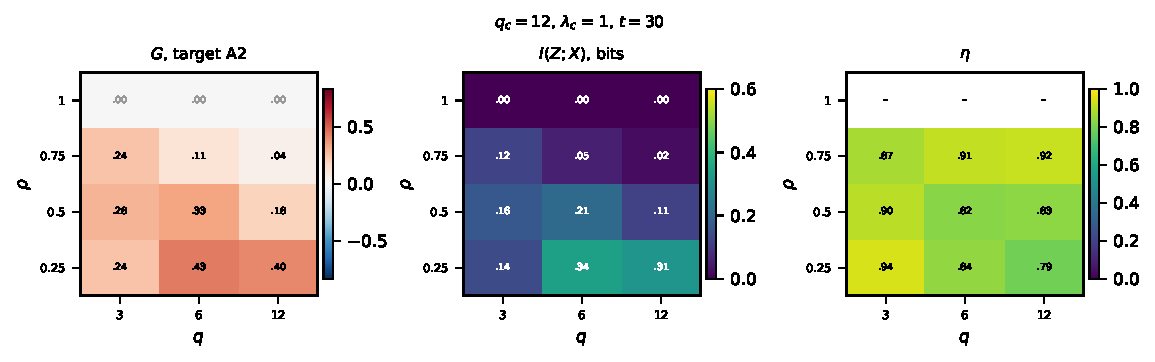
\includegraphics[width=0.98\linewidth]{figures/fig_phase_rho_q.pdf}
\caption{Susceptibility, readability and efficiency over memory $\rho$ and the posts each agent reads $q$;
$q_c = 12$, $\lambda_c = 1$.}
\label{fig:phaserq}
\end{figure}

\begin{itemize}\itemsep1pt
\item \textbf{Reading more defends the proof only when agents remember well}: at $\rho = 0.75$, $G$ falls from
  $0.24$ ($q = 3$) to $0.04$ ($q = 12$) and $I$ from $0.12$ to $0.02$ bits; at $\rho = 0.25$, $G$ rises from $0.24$ to
  $0.40$--$0.43$ ($q = 6$, 12) and $I$ from $0.14$ to $0.31$--$0.34$. A likely reason, not tested: with heavy
  forgetting the proof cannot be rebuilt anyway, and reading more only spreads the controller's facts faster.
\item \textbf{$\eta$ stays at 0.79--0.94} across this whole reversal.
\end{itemize}

\begin{figure}[H]
\centering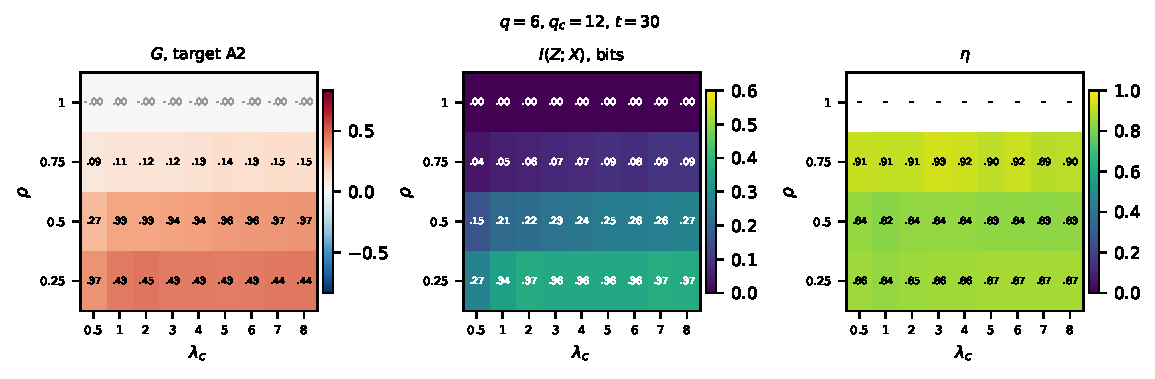
\includegraphics[width=0.98\linewidth]{figures/fig_phase_rho_x.pdf}
\caption{Susceptibility, readability and efficiency over memory $\rho$ and the controller rate $\lambda_c$;
$q = 6$, $q_c = 12$.}
\label{fig:phaserx}
\end{figure}

\begin{itemize}\itemsep1pt
\item \textbf{Memory sets the level, the rate barely changes it}: $G$ goes from 0 at $\rho = 1$ to $0.37$--$0.45$ at
  $\rho = 0.25$; along each row it changes by at most $0.10$, almost all of it between $\lambda_c = 0.5$ and 1.
\item \textbf{$G$ and $I$ move together} (rows ordered the same way; $I$ from $0.04$ to $0.37$ bits); \textbf{$\eta$
  does not} (0.82--0.93, highest at $\rho = 0.75$ where the effects are smallest).
\end{itemize}

\begin{figure}[H]
\centering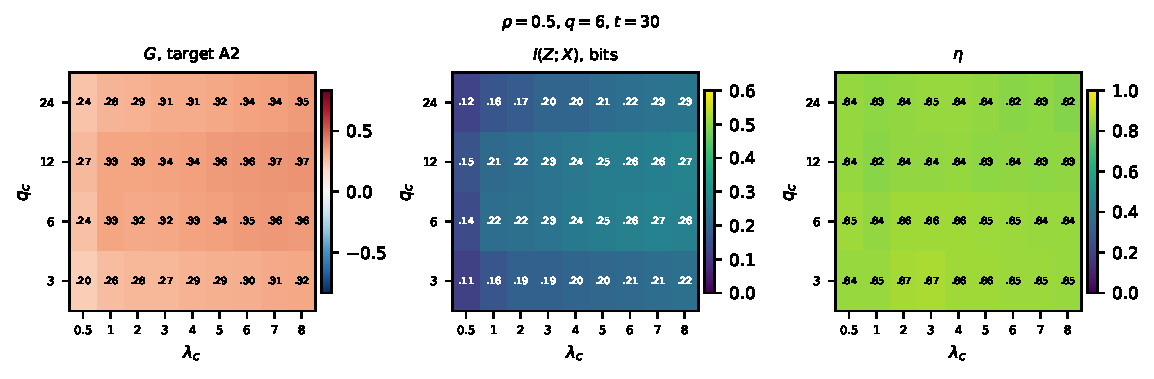
\includegraphics[width=0.98\linewidth]{figures/fig_phase_qc_x.pdf}
\caption{Susceptibility, readability and efficiency over the posts the controller reads $q_c$ and its rate
$\lambda_c$; $\rho = 0.5$, $q = 6$.}
\label{fig:phaseqx}
\end{figure}

\begin{itemize}\itemsep1pt
\item \textbf{The controller's reading budget matters little}: mean $G$ $0.28$, $0.33$, $0.34$, $0.31$ for
  $q_c = 3, 6, 12, 24$; $I$ within $0.11$--$0.27$ bits; $\eta$ within $0.82$--$0.87$.
\item \textbf{Above $\lambda_c = 1$ little changes} along any row ($G$ by at most $0.07$), in any of the three
  observables: the budget is spent before $t = 30$.
\end{itemize}

\section{Susceptibility against the rate, and its slope}\label{sec:strength}

\begin{figure}[H]
\centering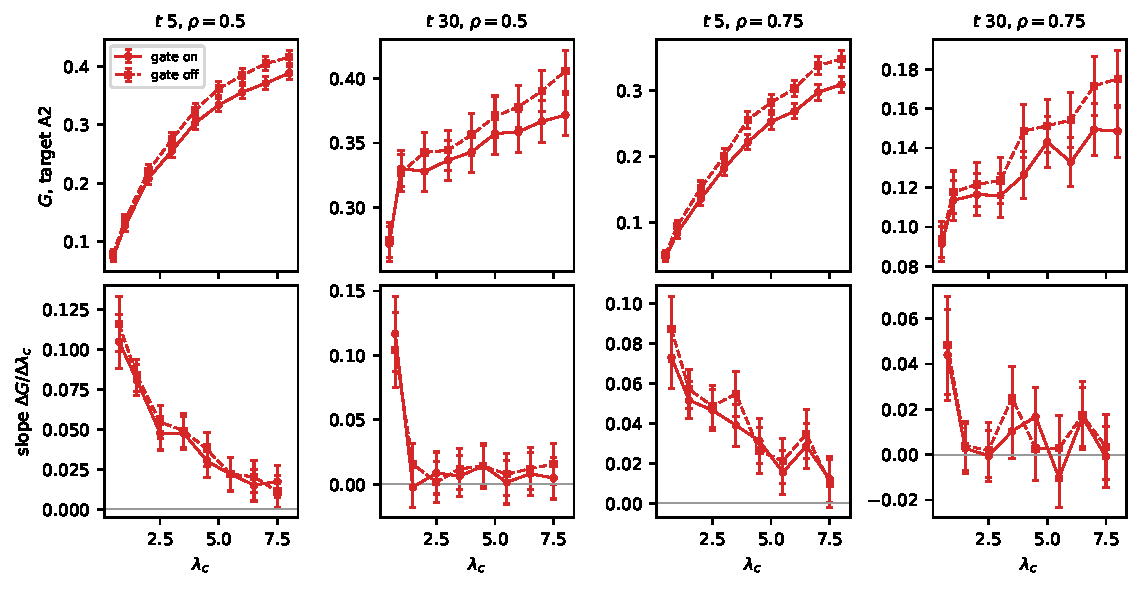
\includegraphics[width=0.95\linewidth]{figures/fig_gain_strength.pdf}
\caption{Top: $G$, target A2, against the controller rate $\lambda_c$, at $t = 5$ and $t = 30$ for $\rho = 0.5$
and $0.75$; gate on (solid) and off (dashed); bars: 95\% intervals. Bottom: the slope between neighbouring rates,
Eq.~(\ref{eq:slope}).}
\label{fig:strength}
\end{figure}

\begin{figure}[H]
\centering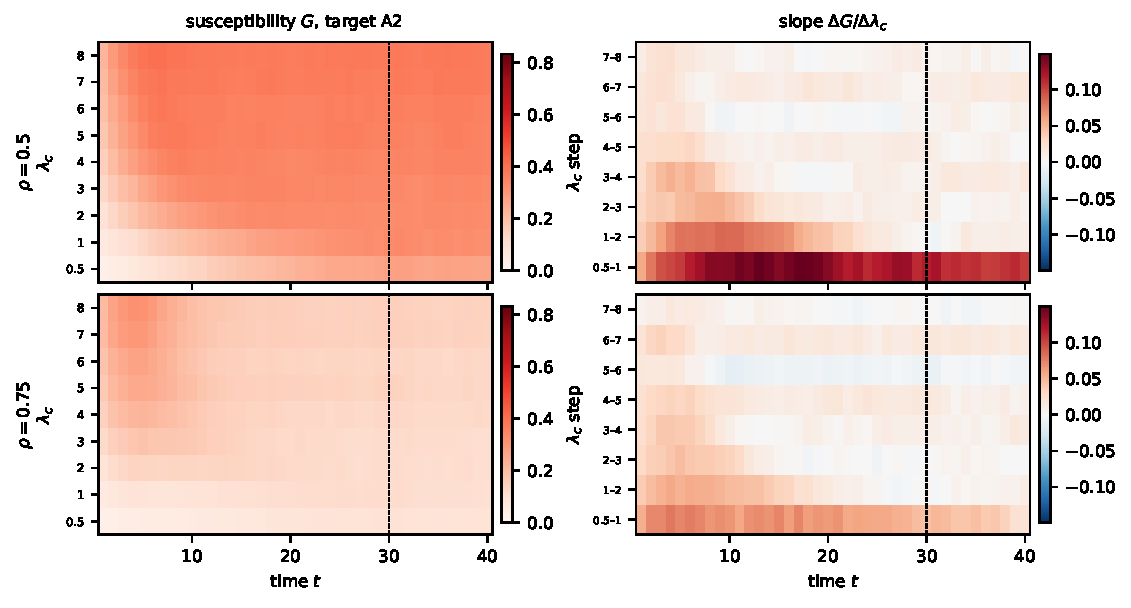
\includegraphics[width=0.95\linewidth]{figures/fig_strength_time.pdf}
\caption{$G$, target A2 (left), and its slope between neighbouring rates (right) over time ($x$) and rate ($y$),
for $\rho = 0.5$ (top) and $0.75$ (bottom); $q = 6$, $q_c = 12$, gate on. Each row of the right panels is one step
between neighbouring rates. The controller stops at $t = 30$ (dashed).}
\label{fig:strengthtime}
\end{figure}

\begin{itemize}\itemsep1pt
\item \textbf{Early, speed buys susceptibility with diminishing returns} (Figure~\ref{fig:strength}): at $t = 5$,
  $\rho = 0.5$, $G$ rises from $0.08$ ($\lambda_c = 0.5$) to $0.39$ ($\lambda_c = 8$); the slope falls from $0.11$
  to about $0.02$ per unit of rate.
\item \textbf{The slope moves down the rate axis as time passes} (Figure~\ref{fig:strengthtime}, right): at
  $\rho = 0.5$, steps above $\lambda_c = 1$ have slopes up to $0.08$ at $t = 5$--10 and at most $0.014$ by $t = 30$;
  only the first step ($0.5 \to 1$) keeps a slope of $0.12$--$0.14$ throughout.
\item \textbf{Fast controllers get there early, slow ones late}: at $\rho = 0.5$, $\lambda_c = 8$ reaches 90\% of its
  $t = 30$ value by $t \approx 3$, $\lambda_c = 0.5$ only by $t \approx 24$ (Figure~\ref{fig:strengthtime}, left).
\item \textbf{The marginal susceptibility is the efficiency of adding rate}: high early and for the first unit of
  rate, close to zero once the budget is spent. Turning the gate off adds at most $+0.03$.
\end{itemize}

\section{Who holds the proof}

\begin{figure}[H]
\centering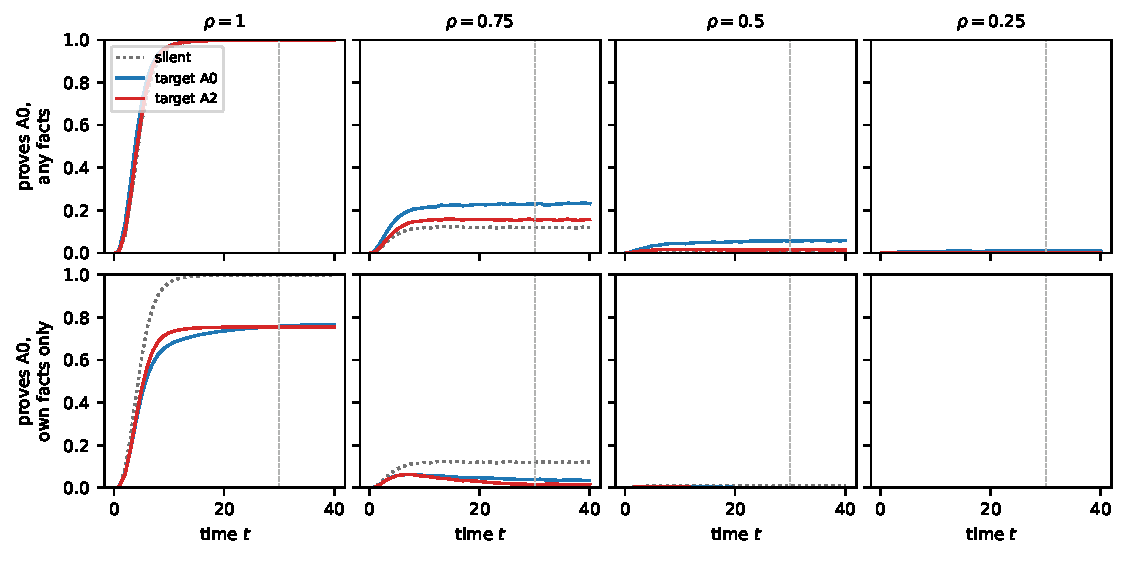
\includegraphics[width=0.95\linewidth]{figures/fig_proofs.pdf}
\caption{Share of agents whose remembered facts prove A0 (top) and prove it from the agents' original facts only
(bottom); silent (dotted), target A0 (blue), target A2 (red); $q = 6$, $q_c = 12$, $\lambda_c = 1$, gate on.}
\label{fig:proofs}
\end{figure}

\begin{itemize}\itemsep1pt
\item \textbf{Proofs need memory}: at $t = 30$ the silent swarm has 100\%, 12\%, 1\% and 0\% of agents proving A0
  for $\rho = 1, 0.75, 0.5, 0.25$. Below $\rho = 0.75$ votes rest on beliefs, not proofs.
\item \textbf{Every controller replaces the agents' own proofs}: with full memory all agents prove A0 under any
  arm, but only 76\% from their own facts under either controller (100\% in silence); at $\rho = 0.75$, 23\% prove A0
  under the truth controller but only 4\% from their own facts.
\item \textbf{The false controller's true facts complete proofs of A0} (16\% against 12\% in silence at
  $\rho = 0.75$).
\end{itemize}

\section{Conclusions}

\begin{enumerate}\itemsep2pt
\item \textbf{Memory decides whether a swarm that owns a proof can be steered.} With full memory every effect
  vanishes by $t \approx 10$. As memory shortens the silent swarm holds the truth less firmly (100\%, 85\%, 71\%,
  58\% voting A0 at $t = 30$) and the susceptibility rises steadily.
\item \textbf{Susceptibility and readability move together; efficiency does not.} In every time series and every
  phase diagram, $G$ and $I$ rise, fall and reverse together, while $\eta$ stays at 0.76--0.94: it measures how
  symmetric the two controllers' effects are, not how large.
\item \textbf{The budget sets the end point; the rate sets the speed.} The slope of $G$ against the rate is large
  early and for the first unit of rate, and close to zero by $t = 30$; per fact, slow control is the most effective.
\item \textbf{The posts each agent reads switch sides with memory}: they defend the proof at $\rho = 0.75$ and help
  the controller at $\rho = 0.25$, in susceptibility and readability alike.
\item \textbf{Control replaces the agents' own proofs}, even when every agent ends up proving the truth.
\item \textbf{Compared with Simulation 1} (same settings, about the same facts posted): Simulation 2 is less
  susceptible at $\rho = 0.5$ (0.33 against 0.53, target A2) and more at $\rho = 0.25$ (0.43 against 0.31).
\end{enumerate}

\paragraph{Caveats.} One world, 24 exact-Bayesian agents voting by probability matching, one controller policy
with a 30-message budget; 1{,}000 episodes per setting (95\% intervals on $G$ about $\pm0.02$). Information is
plug-in from 1{,}000 episodes per arm. Data:
\texttt{results/simulation\_2/2026-10-15\_sim2\_symmetric\_fine}; tables and figures:
\texttt{analysis/task003\_llm\_free/symmetric\_fine/}.

\end{document}
